\documentclass[border=2pt]{standalone}
\usepackage[dvipsnames,svgnames,x11names]{xcolor}
\usepackage{tikz}
\usetikzlibrary{arrows.meta,backgrounds,fit}
\begin{document}
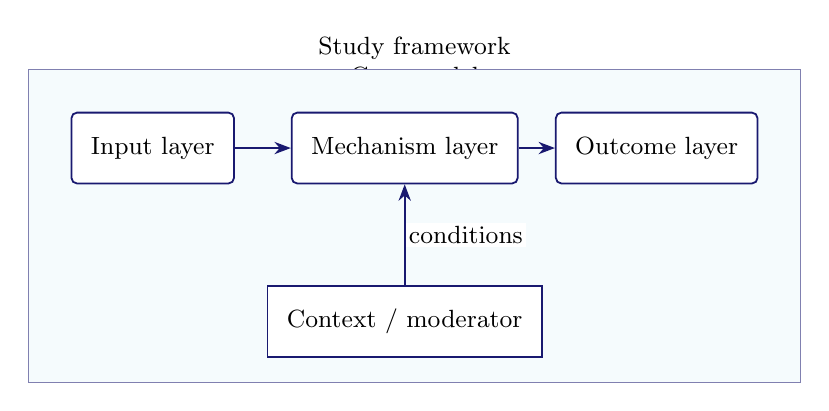
\begin{tikzpicture}[font=\small,>=Stealth,x=32mm,y=22mm]
\node[rectangle,rounded corners=2pt,fill=white,draw=MidnightBlue,text=black,line width=0.65pt,minimum height=9mm,inner xsep=7pt,inner ysep=4.5pt,align=center] (input) at (0,0) {Input layer};
\node[rectangle,rounded corners=2pt,fill=white,draw=MidnightBlue,text=black,line width=0.65pt,minimum height=9mm,inner xsep=7pt,inner ysep=4.5pt,align=center] (process) at (1,0) {Mechanism layer};
\node[rectangle,rounded corners=2pt,fill=white,draw=MidnightBlue,text=black,line width=0.65pt,minimum height=9mm,inner xsep=7pt,inner ysep=4.5pt,align=center] (outcome) at (2,0) {Outcome layer};
\node[rectangle,fill=white,draw=MidnightBlue,text=black,line width=0.65pt,minimum height=9mm,inner xsep=7pt,inner ysep=4.5pt,align=center] (moderator) at (1,-1) {Context / moderator};
\begin{scope}[on background layer]
\node[fit=(input)(process)(outcome),inner sep=6pt,fill=SkyBlue!8,draw=MidnightBlue!55,line width=0.5pt,label={[font=\small]above:{Core model}}] (core) {};
\node[fit=(core)(moderator),inner sep=9pt,fill=SkyBlue!8,draw=MidnightBlue!55,line width=0.5pt,label={[font=\small]above:{Study framework}}] (system) {};
\end{scope}
\draw[->,draw=MidnightBlue,line width=0.65pt] (input) -- (process);
\draw[->,draw=MidnightBlue,line width=0.65pt] (process) -- (outcome);
\draw[->,draw=MidnightBlue,line width=0.65pt] (moderator) -- node[pos=0.5,right,fill=white,inner sep=1.2pt] {conditions} (process);
\end{tikzpicture}
\end{document}
